% ==========================================================================
\section{Computer Maintenance}
% ==========================================================================

    % ==========================================================================
    \subsection{Internal Battery}
    % ==========================================================================

    While it is unplugged from the main power or switched off, the computer
    keeps the date and time, thanks to its Real-Time Clock (RTC) internal
    circuitry.

    This RTC is supported by a LIR2032 Li-Ion rechargeable 3.6V button cell
    battery in the dastaz80 original, and a CR2016 non-rechargeable 3V button
    cell battery in the dastaZ80DB.

    For the LIR2032, to maintain the battery at full charge, ideally the
    computer SHOULD be switched ON for at least one hour every month.
    Nevertheless, after a few years, due the way rechargeable batteries work,
    the battery may be unable to recharge anymore. In such case, the baterry
    MUST be replaced with a new battery of the same characteristics.

    In the case of the CR2016, the battery charge will be consumed after a
    certain number of hours of use, independently of how often or long the
    computer is powered ON.

    In any case, if you are not planning to use the computer for a year or more,
    it is highly recommended to remove the battery, to avoid leaking of chemical
    fluids that are highly toxic and also can damage the internal circuitry.

    There is no danger of electrical shock, as the computer is powered just by
    12V max., but it is highly recommended to unplug the computer to avoid
    possible short circuits that could damage the internal circuitry. It is also
    recommened to discharge yourself from static electricity before touching the
    inside of the computer.

        % ==========================================================================
        \subsubsection{dastaZ80 Original}
        % ==========================================================================

        To replace/remove the battery you need to open the computer case, by
        unscrewing the three small cross-head screws under the front edge of
        the computer case.

        \centerline{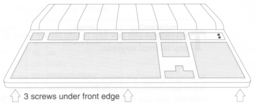
\includegraphics[scale=1]{images/keyboardscrews.png}}

        You can use either a rechargeable LIR2032 battery or a non-rechargeable
        CR2016.

        % ==========================================================================
        \subsubsection{dastaZ80DB}
        % ==========================================================================

        To replace/remove the battery you need to open the computer case, by
        lifting the cover from the left side of the computer.

        You MUST use only a non-rechargeable CR2016 battery.

    % ==========================================================================
    \subsection{Environment and Cleaning the computer}
    % ==========================================================================

    In general, avoid high humidity, extreme cold, and extreme heat
    environments... and do not put the computer in the dishwasher!

    For the dastaZ80, it is highly recommended to use a cover to avoid the
    concentration of dust in the keyboard, which can lead to false contacts.

    The dastaZ80DB has an internal fan that will blow air to the outside when a
    certain temperature inside the box has been reached. To ensure a good flow
    of air, ensure there is a good gap between the back of the computer and any
    object behind the computer.

    Before switching ON the dastaZ80DB, if you see a blinking exclamation mark
    on the Page 0 (as explained in section \hyperref[subsubsec:controlpanel]
    {Control Panel}) DO NOT switch the computer ON until it cooled down.